\documentclass[12pt]{article}

\usepackage{graphicx}
\usepackage{hyperref}
\usepackage{float}

\title{Práctica 1 - Algoritmos Genéticos - SSII}
\date{21 de Octubre, 2026}
\author{Ángel Ruiz Fernandez \and Yingxuan Wang}

\begin{document}

    \maketitle
    \pagebreak

    \tableofcontents
    \pagebreak

    \section{Explicación de Algoritmo Genético}

    \subsection{Elementos}

    \begin{itemize}
    \item \textbf{Representación:} cómo mediante simbolos, el algoritmo entiende la información
     correspondiente al mundo real o espacio de la solución
    \item \textbf{Operadores:} cambian el estado, mediante ellos se llega a la solución. algunos
     pasos se acercan a la solución y otros se alejan
    \item \textbf{Estrategia del control:} cuando aplicar que operadores, de manera que nominalmente
     se encamine hacia una solución
    \end{itemize}

    \subsection{Representación}

    \subsubsection{Codificación}

    Representación del estado, o cromosoma.

    Dependiendo del problema se usan distintos tipos de elemento (gen): binario, entero, real, orden...

    \subsubsection{Operadores genéticos}

    \begin{itemize}
    \item \textbf{Selección:} escoge que individuos van a reproducirse y cuales no
        \begin{itemize}
        \item \textbf{Ruleta:} probabilidad de ser seleccionado proporcional a su función idoneidad
        \item \textbf{Torneo:} se celebran n torneos de parejas de individuos donde ganan por idoneidad
        \end{itemize}
    \item \textbf{Cruce:} el acto de combinar los cromosomas para producir descendencia
        \begin{itemize}
        \item Por punto
        \item Por dos puntos
        \end{itemize}
    \item \textbf{Mutación:} con cierta probabilidad, el cromosoma varía de cierta manera
        \begin{itemize}
        \item Cambio de gen aleatorio (bit flip)
        \item Intercambio de genes
        \end{itemize}
    \end{itemize}

    \subsubsection{Algoritmo genético}

    \begin{itemize}
    \item Seleccionar k elementos
    \item De ellos, con probabilidad $P_c$ se cruzan individuos, la descendencia reemplaza a los padres
    \item Con probabilidad $P_m$, se muta cualquiera de los individuos
    \end{itemize}

    \subsection{Proceso}

    Diseño y construcción de un algoritmo genético

    \begin{enumerate}
    \item Diseñar una representación apropiada para el espacio de soluciones
    \item Decidir cómo inicializar una población. Uniforme para cubrir todos los máximos locales, o heurística previa
    \item Diseñar una correspondencia entre genotipo y fenotipo. A veces la correspondencia es directa; otras el genotipo es la entrada de algún algoritmo clásico que genera la solución final.
    \item Diseñar una forma de evaluar un individuo. Función de idoneidad (fitness) que distinga los genotipos mas adaptados y menos.
    \item Decidir cómo seleccionar los individuos para ser padres. Situar la linea entre los que se reproducen y los que no.
    \item Diseñar un operador de cruce adecuado. Intensificar. Probabilidad alta ($0.6 < P_c < 0.9$), debe hacer heredar características de los padres, no crear otras nuevas.
    \item Diseñar un operador de mutación adecuado. Diversificar. Probabilidad baja ($P_m$), lo suficientemente significativa como para alcanzar todo el espacio de busqueda.
    \item Decidir la condición de parada. Determinada por una función que comprueba si se ha llegado a una solución (óptima?).
    \end{enumerate}

    \section{Analisis}

    El estudio inicial del documento ``P1.2-Fundamentos-Practicos.pdf'' estableció las bases del ajuste de parámetros. En este nuevo análisis, partimos de dichas decisiones previas para los casos de menor dimensión, pero las extendemos y adaptamos para cubrir el rango completo de 8 a 70 reinas.\\\\
    El sistema, para 10000 generaciones, operador de cruce por un punto, operador de mutación ``Flipmutador'' y utilizando los casos para el ajuste de tamaños 8-40, tiene su mejor comportamiento con:

\begin{itemize}
    \item \textbf{Operador de selección TOUR:} Observando las tablas de los operadores de selección TOUR y ROUL, vemos que TOUR tiene un mejor comportamiento al conseguir 0 jaques para más casos, que es el resultado óptimo que esperamos.
    \item \textbf{Tamaño de población 100:} Centrándonos en los resultados de la tabla de TOUR, para el tamaño de población fijamos el valor 100 en vez de 150. A pesar de que tienen un comportamiento similar, como la complejidad en espacio y en tiempo dependen del tamaño de la población, al elegir un valor menor aseguramos que el programa ocupa menos memoria.
    \item \textbf{Pc = 0.85:} Para los parámetros Pc = 0.85 y Pc = 0.9, el sistema tiene un comportamiento similar, obteniendo valores 0 en prácticamente los mismos casos. Según la complejidad en tiempo, seleccionamos 0.85 por requerir menos recursos, ya que al tener una probabilidad de cruce ligeramente más baja, realiza menos cruces y mejora el tiempo.
    \item \textbf{Pm:} El comportamiento de Pm nos induce que conforme vamos teniendo mayor número de reinas el valor de Pm debería decrecer. Seleccionamos 0.05 para \(nreinas \leq 8\) y 0.025 para \(9 \leq nreinas \leq 40\). Esto se debe a que con esos valores cada caso obtiene el resultado óptimo de 0 jaques, y son de los valores más pequeños que se pueden usar con menos recursos, al reducir la probabilidad de mutación se realizan mejores operaciones y mejora el tiempo.
\end{itemize}
De 41 hasta 70 reinas, la probabilidad de mutación de 0.05 a 0.025 anterior es demasiado alta para asegurar una solución óptima (0 jaques). Entonces en este nuevo estudio se añaden columnas de 0.01375 y 0.0125, en las que aparecen más soluciones a lo largo de toda la dimensión de N de reinas.\\
Analizando los resultados:
\begin{itemize}
    \item El valor Pm = 0.01375 obtiene un fitness de 0 de forma continua para \(29 \leq nreinas \leq 67\), pero falla (fitness=1) en nreinas=68.
    \item El valor Pm = 0.0125 falla en nreinas=61, pero obtiene 0 en el resto de casos.
\end{itemize}
Para obtener un mejor comportamiento con los menos recursos posibles, hemos mantenido las decisiones para \(nreinas \leq 28\), y elegimos Pm = 0.01375 para N reinas de 29 a 61, y Pm = 0.0125 de 62 a 70. De esta forma, se evitan las instancias donde el algoritmo genético no llega a una solución satisfactoria, se mantiene el patrón de que conforme crece el problema (mayor número de reinas) decrece el valor de Pm, y se garantiza que tarde el menor tiempo posible en llegar a una solución.

    \section{Manual de Asignación}

    \begin{enumerate}
    \item \textless N de reinas \textgreater
    \item Valor para el párametro 2º: 100 (valor recomendado)
    \item Valor para el párametro 3º: 10000 (valor recomendado)
    \item Valor para el párametro 4º: TOUR (valor recomendado)
    \item Valor para el párametro 5º: ONEP (valor recomendado)
    \item Valor para el párametro 6º: FLIP (valor recomendado)
    \item Valor para el párametro 7º: 0.85 (valor recomendado)
    \item Valor para el párametro 8º: para N reinas
        \begin{itemize}
           \item \textless= 8: 0.05 (valor recomendado)
           \item {[9, 28]}: 0.025 (valor recomendado)
           \item {[29, 61]}: 0.01375 (valor recomendado)
           \item {[62, 70]}: 0.0125 (valor recomendado)
       \end{itemize}
    \end{enumerate}

    \section{Validación}

    Casos de validación

    Ejecución: \texttt{./nreinas <N reinas> <2> <3> <4> <5> <6> <7> <8>}

    \begin{table}[H]
    \centering
    \begin{tabular}{|| c c c c c c c c | c ||}
    \hline
    N reinas & 2 & 3 & 4 & 5 & 6 & 7 & 8 & jaques \\ [0.5ex]
    \hline
    \hline
    7 & 100 & 10000 & TOUR & ONEP & FLIP & 0.85 & 0.05 & 0 \\
    8 & 100 & 10000 & TOUR & ONEP & FLIP & 0.85 & 0.05 & 0 \\
    23 & 100 & 10000 & TOUR & ONEP & FLIP & 0.85 & 0.025 & 0 \\
    28 & 100 & 10000 & TOUR & ONEP & FLIP & 0.85 & 0.025 & 0 \\
    40 & 100 & 10000 & TOUR & ONEP & FLIP & 0.85 & 0.01375 & 0 \\
    41 & 100 & 10000 & TOUR & ONEP & FLIP & 0.85 & 0.01375 & 0 \\
    61 & 100 & 10000 & TOUR & ONEP & FLIP & 0.85 & 0.01375 & 0 \\
    68 & 100 & 10000 & TOUR & ONEP & FLIP & 0.85 & 0.0125 & 0 \\
    72 & 100 & 10000 & TOUR & ONEP & FLIP & 0.85 & 0.0125 & 0 \\
    73 & 100 & 10000 & TOUR & ONEP & FLIP & 0.85 & 0.0125 & 0 \\
    \hline
    \end{tabular}
    \caption{Asignaciones y resultado}
    \end{table}

    Para los anteriores casos de validación se obtiene un resultado favorable

    \section{Analisis del comportamiento global del SI basado en AG con respecto 4 criterios}

    \subsection{Completitud}

   El sistema demuestra una alta completitud para los casos de validación. Dado que el problema de las n-reinas tiene solución para \(n \geq 4\), el AG es capaz de encontrarla en la gran mayoría de los casos antes de alcanzar el límite de 10000 generaciones. La inclusión de un criterio de parada temprano (cuando fitness=0) asegura que el sistema no desperdicie recursos una vez encontrada la solución.

    \subsection{Optimalidad}

    Aunque los Algoritmos Genéticos no garantizan encontrar el óptimo global (es una técnica heurística), nuestro sistema alcanza el fitness 0 (solución óptima) en la gran mayoría de los casos gracias al ajuste de parámetros realizado.

    \subsection{Complejidad en tiempo}
    El coste temporal del sistema depende principalmente del tamaño de la población (TP=100), el número máximo de generaciones (10000) y el coste de evaluar la función fitness. Con mayor número de reinas más tarda el sistema en encontrar una solución.\\La función Objective tiene una complejidad de \(O(n^2)\) debido al doble bucle que comprueba los ataques. Además, hemos optimizado el tiempo al elegir TP=100 (en lugar de 150), Pc=0.85 (en lugar de 0.9) y los valores menor posibles de Pm para cada caso, así reduciendo el número de operaciones por generación sin perder calidad en las soluciones.
    \begin{table}[H]
    \centering
    \begin{tabular}{|| c c ||}
    \hline
    N reinas & tiempo (s) \\ [0.5ex]
    \hline
    \hline
    7 & 0.011 \\
    8 & 0.006 \\
    23 & 0.042 \\
    28 & 0.877 \\
    40 & 2.182 \\
    41 & 0.571 \\
    61 & 5.676 \\
    68 & 4.077 \\
    72 & 12.294 \\
    73 & 15.975 \\
    \hline
    \end{tabular}
    \caption{Tabla de tiempos}
    \end{table}

    \begin{figure}[H]
    \centering
    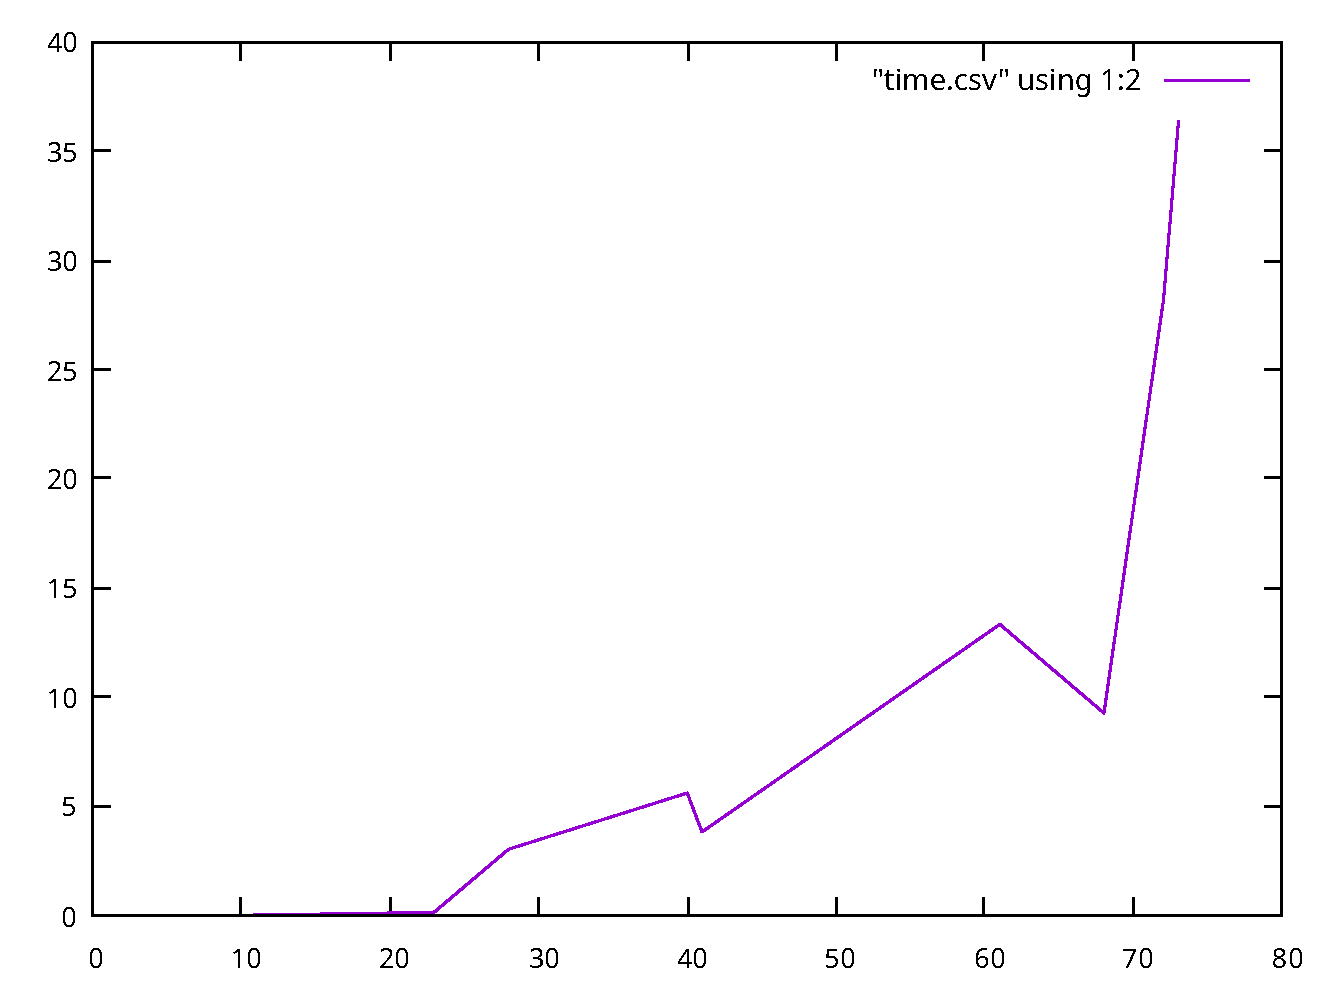
\includegraphics[width=0.5\textwidth]{time}
    \caption{Grafico de tiempos}
    \end{figure}

    \subsection{Complejidad en memoria}

    El consumo de memoria está directamente relacionado con el tamaño de la población. Al fijar el tamaño de la población en 100, garantizamos que el espacio requerido sea reducido y constante.

\end{document}